\documentclass{article}
\usepackage{graphicx} % Required for inserting images
\usepackage{tikz}
\usetikzlibrary{positioning}
\title{presentation_graphics_cis5200}
\author{sunggun }
\date{December 2025}

\begin{document}


\begin{table}[h]
\centering
\begin{tabular}{lcc}
\hline
\textbf{Statistic} & \textbf{Value} \\
\hline
Number of reviews & 105{,}998 \\
Number of products & 11{,}701 \\
Average reviews per product & $\approx 9$ \\
Image review percentage & $8.2\%$ \\
Median inter-review time & $3.2$ days \\
Mean inter-review time & $10.7$ days \\
Supervised rows (after censoring) & 94{,}297 \\
\hline
\end{tabular}
\caption{Dataset overview for Amazon Appliances reviews (Jan--Jun 2023).}
\end{table}


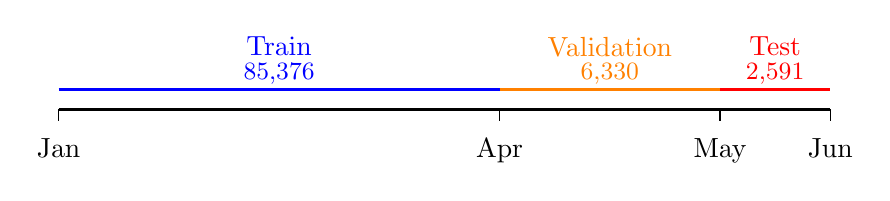
\begin{tikzpicture}[x=0.7cm,y=1cm]

  % Main axis
  \draw[thick] (0,0) -- (14,0);

  % Ticks + labels
  \foreach \x/\m in {0/Jan,8/Apr,12/May,14/Jun} {
    \draw (\x,0) -- (\x,-0.15);
    \node[below] at (\x,-0.25) {\m};
  }

  % --- Train Segment (Jan–Apr) ---
  \draw[very thick,blue] (0,0.25) -- (8,0.25);
  \node[blue] at (4,0.8) {\medium Train};
  \node[blue] at (4,0.45) {\small 85{,}376};

  % --- Validation Segment (Apr–May) ---
  \draw[very thick,orange] (8,0.25) -- (12,0.25);
  \node[orange] at (10,0.8) {\medium Validation};
  \node[orange] at (10,0.45) {\small 6{,}330};

  % --- Test Segment (May–Jun) ---
  \draw[very thick,red] (12,0.25) -- (14,0.25);
  \node[red] at (13, 0.8) {\medium Test};
  \node[red] at (13,0.45) {\small 2{,}591};

\end{tikzpicture}
\[
y_{\log} = \log\!\left(1 + \mathrm{hours\_to\_next\_review}\right)
\]
\[
y_{\text{hours}} = \mathrm{hours}(\Delta t_i)
\qquad
y_{\log} = \log(1 + y_{\Delta t_i}) \]

$y_{\Delta t_i} = t_{i+1} - t_{i} \] 



\end{document}
